	\documentclass[aps,prx,twocolumn,superscriptaddress,showpacs]{revtex4-1}
\usepackage{amsmath,amssymb,graphicx}

\usepackage[utf8]{inputenc}
\usepackage[T1]{fontenc}
\usepackage{xcolor}

\newcommand{\comment}[1]{\textcolor{blue}{\textbf{#1}}}
\IfFileExists{newtxtext.sty}
   {\usepackage{newtxtext,newtxmath}}
   {\IfFileExists{stix.sty}
      {\usepackage{stix}}
      {\IfFileExists{mathptmx.sty}
      {\usepackage{mathptmx}}{} } }

\usepackage{textcomp}
\newcommand\bmmax{2}
\usepackage{bm}

\IfFileExists{siunitx.sty}{\usepackage{booktabs,siunitx}}{}

\pdfoutput=1
\usepackage{color}
\definecolor{LinkColor}{rgb}{0.256,0.439,0.588}
\usepackage{hyperref}
\hypersetup{
   pdfauthor={F. F. Assaad},
   pdftitle={},
   %pdfsubject={SUBJECT},
   %pdfkeywords={KEYWORDS1,} {KEYWORDS2,} {KEYWORDS3,} {KEYWORDS4},
   colorlinks=true,
   citecolor=LinkColor,
   linkcolor=LinkColor,
   urlcolor=LinkColor
}

\usepackage{pifont}


\usepackage{epstopdf}

\begin{document}


\title{ Documentation and definition of the model  }

\author{ F.F. Assaad}
\affiliation{Institut f\"ur Theoretische Physik und Astrophysik, Universit\"at W\"urzburg, 97074 W\"urzburg, Germany}

\date{\today}

\begin{abstract}

\end{abstract}

\pacs{71.10.-w,71.10.Hf,75.40.Cx,75.40.Mg}

\maketitle

The Hamiltonian is defined as: 
\begin{widetext}
\begin{equation}
	-t \sum_{ \langle \pmb{i},\pmb{j} \rangle  \sigma}   \left( \hat{c}^{\dagger}_{\pmb{i},\sigma} \hat{c}_{\pmb{j}, \sigma} + H.c. \right)  +
	  J \sum_{\pmb{i}} \hat{\pmb{S}}^{c}_{\pmb{i}} \cdot \hat{\pmb{S}}^{f}_{\pmb{i}}  +  
	  4  I_z  \sum_{ \langle \langle \pmb{i},\pmb{j} \rangle \rangle  }  \hat{S}^{f,z}_{\pmb{i}}   \hat{S}^{f,z}_{\pmb{j} }
 \end{equation}

\begin{figure*}[h]
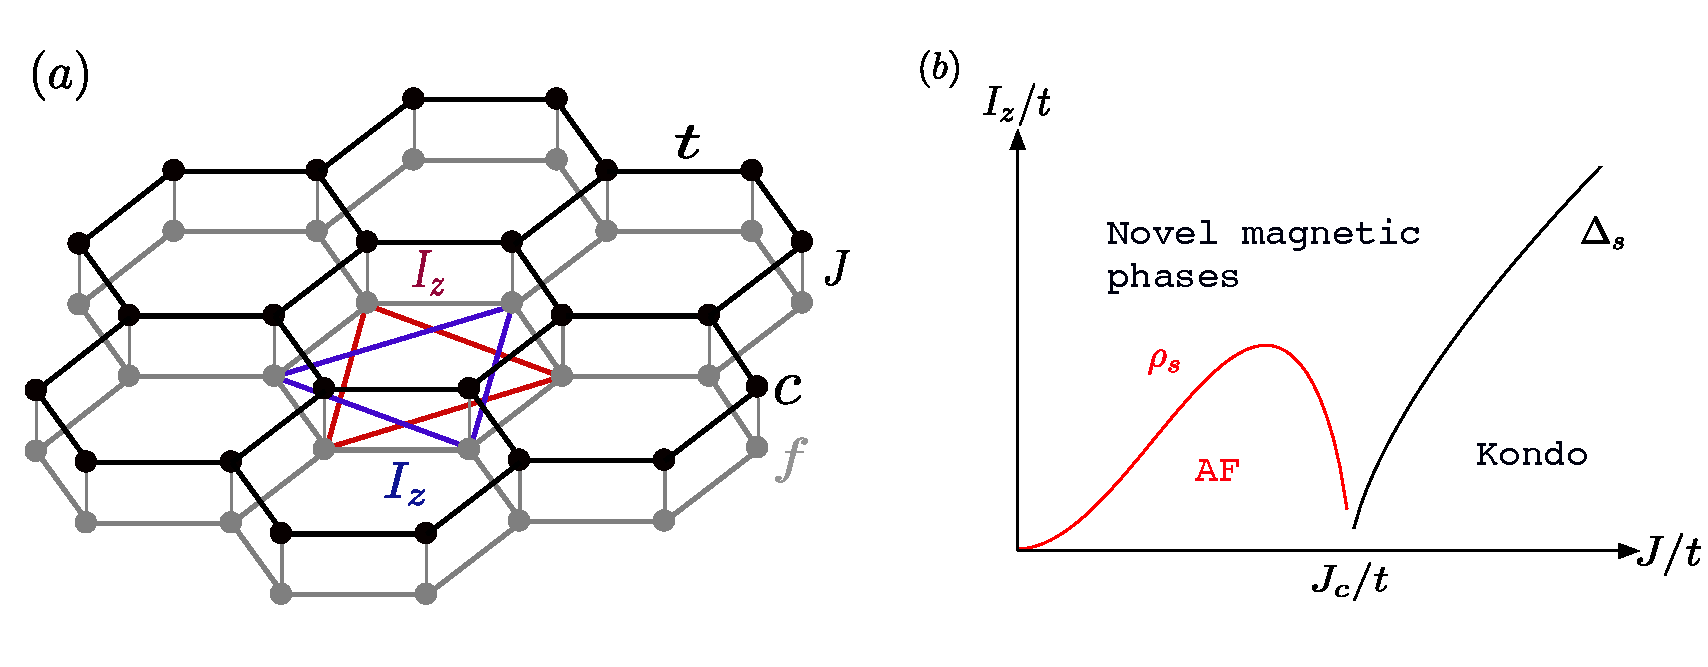
\includegraphics[width=0.99\linewidth]{Kondo1.pdf}
\end{figure*}
\end{widetext}
\end{document}
